\chapter{Experiments and Results}
\label{chap:Experiments and Results}
%-------------------------------------------------------------------
This chapter will provide information about the experiments that were capable of changing the Hadoop scheduling behavior and the results achieved.

\section{Collector integration test}
This experiment had the objective of testing the collector integration. The experiment consisted in deploying and starting Hadoop services in the cluster with original CapacityScheduler and with the context-aware CapacityScheduler in order to compare the change in total resources availability.

\subsection{Hardware and Software configuration}
The experiment was performed in a cluster deployed on Grid'5000 environment. The cluster had five nodes, one master and four slaves, each node having the following configuration: 2 CPUs AMD@1.7GHz, 12 cores/CPU and 47GB RAM. All nodes were running an Ubuntu-x64-1204 standard image, having Sun JDK 1.7 installed. The Hadoop distribution was the 2.2.0 YARN version.

The default Hadoop configuration is set on \textit{yarn-default.XML} under the properties named \textit{yarn.nodemanager.resource.memory-mb} and \textit{yarn.nodemanager.resource.CPU-vcores} which have default values of 8192 and 8 respectively. The only difference being that one of the executions had the collector plugged.

\subsection{Procedures}
The procedure chosen as data acquisition method was the Hadoop Log System. The reason for such a choice was that Hadoop Log System is, by default, enabled in the INFO level and using the INFO level would be possible to insert small entries and extract useful information in real time. The data was acquired with the same call during the execution of services with both schedulers.

\subsection{Results and interpretation}
The comparison of node memory from default and collector implementation can be seen in the table \ref{tab:experiments}.

\begin{table}
\renewcommand{\figurename}{Table}
\centering
\begin{tabular}{|c|c|c|}
\hline 
  & Original CapacityScheduler & Context-aware CapacityScheduler \\ 
\hline 
Node Memory & 8192 & 48303 \\ 
\hline 
Node Vcores & 8 & 24 \\ 
\hline 
\end{tabular}
\caption{Resources available on original and context-aware CapacityScheduler}
\label{tab:experiments}
\end{table}

There are also two more figures that express how better the collector implementation scales given proper hardware. These figures are figure \ref{fig:experiment2} and figure \ref{fig:experiment3}.

\begin{figure}[!hbtn]
   \renewcommand{\figurename}{Figure}
   \centering
   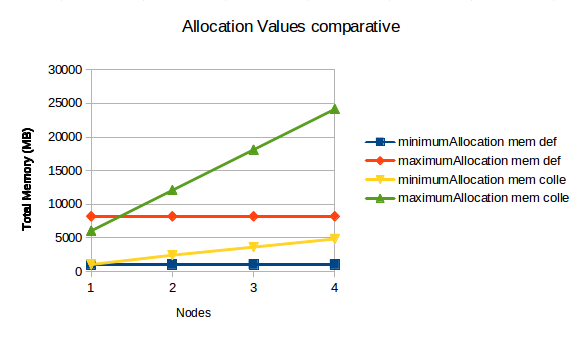
\includegraphics[width=15cm]{figuras/Figura10-totalMemory.png}
   \caption{Cluster memory available on default and collector implementation}
   \label{fig:experiment2}
\end{figure}

\begin{figure}[!hbtn]
   \renewcommand{\figurename}{Figure}
   \centering
   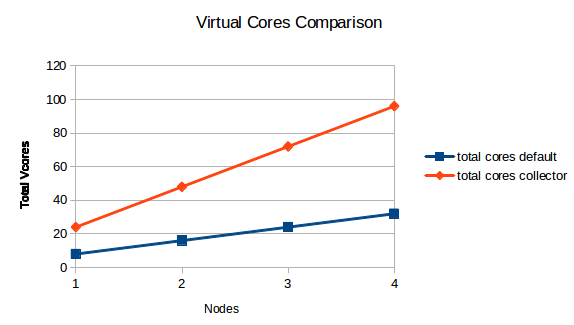
\includegraphics[width=15cm]{figuras/Figura12-totalCores.png}
   \caption{Cluster cores available on default and collector implementation}
   \label{fig:experiment3}
\end{figure}

Since this experiment was run on Grid'5000 and all nodes have the same configuration, it would be easy to discover the true capacity of a node, change the values on a XML file and replicate it to all other nodes inside the environment. The problem becomes huge once the environment is not homogeneous. It would require someone to discover the true capacity of each node and then separately edit the XML files in every node.

Consider that according to HadoopWizard \cite{HadoopWizard} by July 2011 Yahoo! used a 42000 nodes Hadoop Cluster, and on the same month Facebook publicized it runs a 2000 nodes Hadoop cluster. Changing every node configuration manually would be quite challenging, therefore the collectors used would come in hand.

\section{Original CapacityScheduler X Context-aware CapacityScheduler}
This experiment was performed in order to compare the container allocation pattern in the original CapacityScheduler and the context-aware CapacityScheduler. The experiment consisted in executing a TeraSort in the cluster with the original CapacityScheduler and the context-aware CapacityScheduler. This was made in order to compare how the higher resource availability and higher allocation limits impacted the scheduling.

\subsection{Hardware and Software configuration}
The experiment used the same hardware configuration from the previous one. Regarding the Hadoop configuration, there are new properties used. The properties are the minimum and maximum allocation values, which are set in properties stated on section \ref{sec:alloc}. The only difference being that one of the executions had the collector plugged.

\subsection{Procedures}
The procedure chosen as data acquisition method was the Hadoop Log System. The reason for such a choice was that Hadoop Log System is, by default, enabled in the INFO level and using the INFO level would be possible to insert small entries and extract useful information in real time. The data was acquired with the same call during the execution of services with both schedulers.

The application used to test the scheduling was a TeraSort with 5GB data to sort, requesting enough containers and providing enough data to be processed in order to stress the cluster.


\subsection{Results and interpretation}
Before going further into the interpretation of the results, there are some characteristics of jobs that need to be reminded. If the number of reduce tasks parameter isn't set on \textit{mapred-site.XML}, the default value used is 1, making the whole reduce step forced to be executed on only one container.

Another thing to note is that the first allocated container is always the ApplicationMaster, making this container not relevant in grant of resources for MapReduce tasks analysis. Thus both the ApplicationMaster and Reducer container were withdraw from the data analyzed, which was left only with the Map containers. All times are normalized related to the first Map container created.

The cluster configuration achieved with the original CapacityScheduler was: 
\begin{itemize}
	\item Total cluster resource of 32768mb and 32cores
	\item Minimum allocation of 1024mb and 1 core
	\item Maximum allocation of 8192mb and 32 cores.
	\item All Map containers were granted containers of 1024mb and 1 core, the minimum limit.
\end{itemize}


The cluster configuration achieved with the context-aware CapacityScheduler was: 
\begin{itemize}
	\item Total cluster resource of 193210mb and 96cores
	\item Minimum allocation of 4830mb and 2 cores
	\item Maximum allocation of 24151mb and 12 cores
	\item All Map containers were granted containers of 4830mb and 2 cores, the minimum limit.
\end{itemize}

Although a huge difference was achieved by only comparing the resources collected and the allocation limits, the main objective of this work is to impact the scheduling performance in a Hadoop cluster. Therefore, a TeraSort execution was made and the results achieved are discussed below.

The following Gantt Charts are consolidated by resources, which are the NodeManagers. This means that the tasks, in this case portrayed as containers, will be consolidated to the resources they are tied. As stated before, the containers are allocated to a certain NodeManager. The consolidation works in a way that when a separation occurs in the segment, it means that a container has either started or finished on that NodeManager. That implies that many containers will be on more than one segment, and, the numbers inside the segment indicates which containers are running at that moment.

Figure \ref{fig:ganttDefault} portraits the Gantt Chart of the TeraSort with original CapacityScheduler. It is easy to notice that some containers had to wait for the completion of others in order to start processing their tasks.

\begin{figure}[hbtn]
   \renewcommand{\figurename}{Figure}
   \centering
   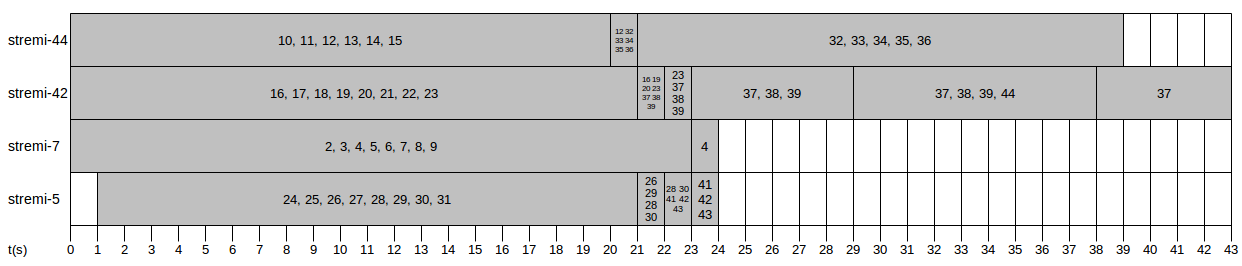
\includegraphics[width=16cm]{figuras/Figura16-GanttDefault.png}
   \caption{Container assignment with default configuration}
   \label{fig:ganttDefault}
\end{figure}

In order to illustrate how to interpret the Gantt charts, the node stremi-42 of figure \ref{fig:ganttDefault} will be taken as example. It starts all its containers, numbered from 16 to 23, at the 0 seconds mark, then the segment ends at the 21 seconds mark, meaning that either a container started or finished. After a quick analysis of the containers in the first and second segments, it is possible to note that containers 17, 18, 21 and 22 are not in the second segment, meaning they have finished processing their tasks. Another thing to notice is that on the second segment, containers with numbers 37, 38 and 39 appeared for the first time, meaning they were started at this time. If the analysis is extended to the segment from 22 to 23 seconds, it is possible to note that containers 16, 19 and 20 have finished processing their tasks too, and the only running containers in this node at this moment are the containers 23, 37, 38 and 39.

Figure \ref{fig:ganttImproved} portraits the Gantt Chart of the TeraSort with context-aware CapacityScheduler. In this case the overall completion time was reduced, this happened due to the fact that all containers could be started right after the arrival of the request, thanks to the higher resource availability.

\begin{figure}[hbtn]
   \renewcommand{\figurename}{Figure}
   \centering
   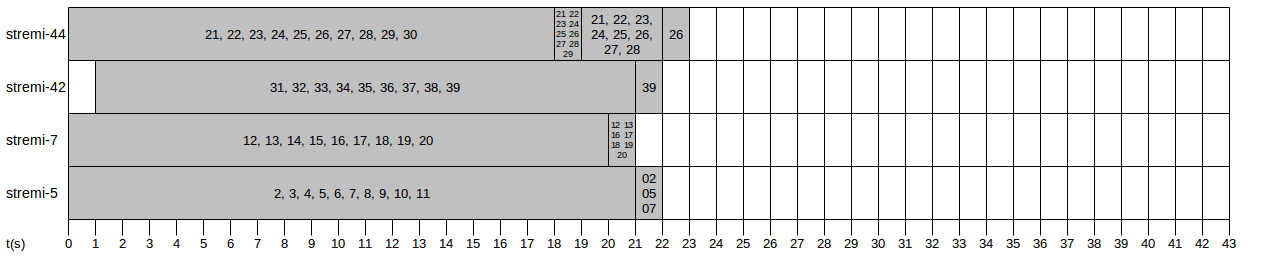
\includegraphics[width=15cm]{figuras/Figura17-GanttImproved.png}
   \caption{Container assignment with the improved configuration}
   \label{fig:ganttImproved}
\end{figure}

After an analysis and comparison of both charts, it is possible to notice that the default chart has containers 41-43 started on node stremi-5 and container 44 started on node stremi-42, while the context-aware chart has only the standard containers, which are numbered 2-39. This happens because these extra containers are, in reality, speculative tasks launched because other tasks were taking to long to finish. Without a better information acquisition it is hard to determine the match of original and speculative containers, but it is possible to infer which containers would make possible candidates, leaving containers 2-9, 23, 28 and 30 as possible staggers, responsible for the launching of speculative containers 41-43. Because of the same reasons, it is only possible to infer that container 44 was launched because the most likely stagger was one container in the 32-36 range.

By analysing the container numberings it is possible to notice how the scheduler decides which node is going to be used. The containers launched on a given node follow a logic numbering, meaning that the resources of that container are used until exhaustion before the scheduler starts launching containers on another node. 

\section{Heterogeneity simulation}
This experiment was performed in order to simulate a heterogeneous environment and test how well would the context-aware would adapt. The experiment consisted in executing a TeraSort in the cluster with the simulated heterogeneous environment using context-aware CapacityScheduler. 

\subsection{Hardware and Software configuration}
The experiment used the same hardware configuration from the previous experiments. Regarding the Hadoop configuration, there are no changes. The only difference is that the nodes are purposely given false capacities when being added to the RM. Using this false values, a heterogeneous cluster will be simulated.

\subsection{Procedures}
The procedure chosen as data acquisition method was the Hadoop Log System. The reason for such a choice was that Hadoop Log System is, by default, enabled in the INFO level and using the INFO level would be possible to insert small entries and extract useful information in real time. The data was acquired with the same call during the execution of services with both schedulers.

The application used to test the scheduling was a TeraSort with 5GB data to sort, requesting enough containers and providing enough data to be processed in order to stress the cluster.

\subsection{Results and interpretation}
As this experiment is a replication of the last one plus the simulated heterogeneity, the same principles applies regarding the container analysis. 

It is important to firstly know the configuration of the simulated heterogeneity. The cluster had the following simulated configuration:

\begin{itemize}
	\item stremi-17: 28981 MB of memory and 14 cores.
	\item stremi-22: 34715 MB of memory and 18 cores.
	\item stremi-33: 46287 MB of memory and 24 cores.
	\item stremi-35: 24151 MB of memory and 12 cores.
	\item Total Cluster Resources: 134134 MB of memory and 68 cores.
	\item Minimum Allocation: 3353 MB of memory and 1 core.
\end{itemize}

Figure \ref{fig:ganttSimulation} portraits the Gantt Chart of the TeraSort execution within the simulated heterogeneous environment, also using context-aware CapacityScheduler. Compared to the default case, the heterogeneous environment execution shows an improvement, but due to the lower cluster capacity, it is a slightly worse than the context-aware CapacityScheduler executing on a homogeneous environment.

\begin{figure}[hbtn]
   \renewcommand{\figurename}{Figure}
   \centering
   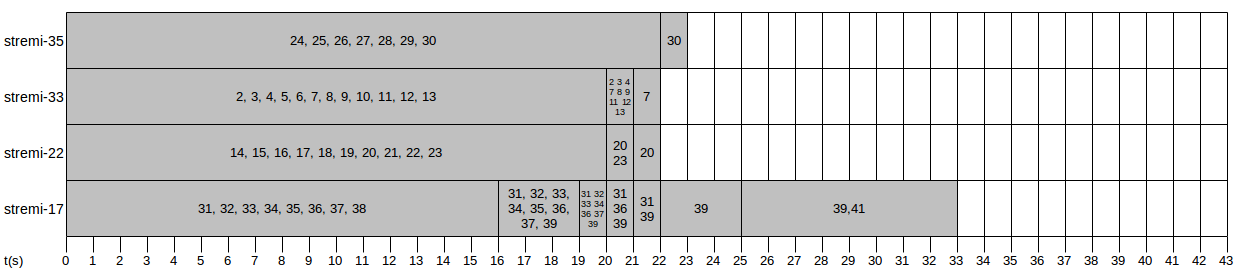
\includegraphics[width=15cm]{figuras/Figura21-GanttSimulation.png}
   \caption{Container assignment with the simulated heterogeneous environment}
   \label{fig:ganttSimulation}
\end{figure}

It is possible to note that the containers started the assignment with the node stremi-33, which is the node with the most capacity in the cluster and also was the first to be added in the node list. As in the other experiments, the scheduler launches containers on a node until its resources are all reserved, then mode to the next node on the list.

On this experiment a speculative task was launched. Contrary to the other experiments, its easy to infer which was the original stagger task, since there was only one container active at the moment that the container 41 was launched. It is also possible to note that the scheduler didn't change nodes to launch the speculative, that happens because the node had spare capacity when the request for the speculative arrived.

This experiment shows that it is possible to use this context-aware in a heterogeneous environment, the allocations were adapted to a slightly smaller cluster if compared to the real environment. As a future work, it is possible to set the allocation limits in function not only of total cluster resources but also of each individual node resource capacity.